%% Преамбула TeX-файла

% 1. Стиль и язык
\documentclass[utf8x, 12pt]{G7-32} % Стиль (по умолчанию будет 14pt)

% Остальные стандартные настройки убраны в preamble-std.tex
\sloppy

% 1. Настройки стиля ГОСТ 7-32
% Для начала определяем, хотим мы или нет, чтобы рисунки и таблицы нумеровались в пределах раздела, или нам нужна сквозная нумерация.
% А не забыл ли автор букву 't' ?
\EqInChapter % формулы будут нумероваться в пределах раздела
\TableInChapter % таблицы будут нумероваться в пределах раздела
\PicInChapter % рисунки будут нумероваться в пределах раздела

% 2. Добавляем гипертекстовое оглавление в PDF
\usepackage[
bookmarks=true, colorlinks=true, unicode=true,
urlcolor=black,linkcolor=black, anchorcolor=black,
citecolor=black, menucolor=black, filecolor=black,
]{hyperref}

% 3. Изменение начертания шрифта --- после чего выглядит таймсоподобно.
% apt-get install scalable-cyrfonts-tex

\IfFileExists{cyrtimes.sty}
    {
        \usepackage{cyrtimespatched}
    }
    {
        % А если Times нету, то будет CM...
    }


% 4. Прочие полезные пакеты.
\usepackage{underscore} % Ура! Теперь можно писать подчёркивание.
                        % И нельзя использовать подчёркивание в файлах.
                        % Выбирай, но осторожно.

\usepackage{graphicx}   % Пакет для включения рисунков

 % 5. Любимые команды
\newcommand{\Code}[1]{\textbf{#1}}

% 6. Поля
% С такими оно полями оно работает по-умолчанию:
% \RequirePackage[left=20mm,right=10mm,top=20mm,bottom=20mm,headsep=0pt]{geometry}
% Если вас тошнит от поля в 10мм --- увеличивайте до 20-ти, ну и про переплёт не забывайте:
\geometry{right=20mm}
\geometry{left=30mm}


% 7. Tikz
\usepackage{tikz}
\usetikzlibrary{arrows,positioning,shadows}

% 8 Листинги

\usepackage{listings}

% Значения по умолчанию
\lstset{
  basicstyle= \footnotesize,
  breakatwhitespace=true,% разрыв строк только на whitespacce
  breaklines=true,       % переносить длинные строки
%   captionpos=b,          % подписи снизу -- вроде не надо
  inputencoding=koi8-r,
  numbers=left,          % нумерация слева
  numberstyle=\footnotesize,
  showspaces=false,      % показывать пробелы подчеркиваниями -- идиотизм 70-х годов
  showstringspaces=false,
  showtabs=false,        % и табы тоже
  stepnumber=1,
  tabsize=4,              % кому нужны табы по 8 символов?
  frame=single
}

% Стиль для псевдокода: строчки обычно короткие, поэтому размер шрифта побольше
\lstdefinestyle{pseudocode}{
  basicstyle=\small,
  keywordstyle=\color{black}\bfseries\underbar,
  language=Pseudocode,
  numberstyle=\footnotesize,
  commentstyle=\footnotesize\it
}

% Стиль для обычного кода: маленький шрифт
\lstdefinestyle{realcode}{
  basicstyle=\scriptsize,
  numberstyle=\footnotesize
}

% Стиль для коротких кусков обычного кода: средний шрифт
\lstdefinestyle{simplecode}{
  basicstyle=\footnotesize,
  numberstyle=\footnotesize
}

% Стиль для BNF
\lstdefinestyle{grammar}{
  basicstyle=\footnotesize,
  numberstyle=\footnotesize,
  stringstyle=\bfseries\ttfamily,
  language=BNF
}

% Определим свой язык для написания псевдокодов на основе Python
\lstdefinelanguage[]{Pseudocode}[]{Python}{
  morekeywords={each,empty,wait,do},% ключевые слова добавлять сюда
  morecomment=[s]{\{}{\}},% комменты {а-ля Pascal} смотрятся нагляднее
  literate=% а сюда добавлять операторы, которые хотите отображать как мат. символы
    {->}{\ensuremath{$\rightarrow$}~}2%
    {<-}{\ensuremath{$\leftarrow$}~}2%
    {:=}{\ensuremath{$\leftarrow$}~}2%
    {<--}{\ensuremath{$\Longleftarrow$}~}2%
}[keywords,comments]

% Свой язык для задания грамматик в BNF
\lstdefinelanguage[]{BNF}[]{}{
  morekeywords={},
  morecomment=[s]{@}{@},
  morestring=[b]",%
  literate=%
    {->}{\ensuremath{$\rightarrow$}~}2%
    {*}{\ensuremath{$^*$}~}2%
    {+}{\ensuremath{$^+$}~}2%
    {|}{\ensuremath{$|$}~}2%
}[keywords,comments,strings]

% Подписи к листингам на русском языке.
\renewcommand*\thelstnumber{\oldstylenums{\the\value{lstnumber}}}
\renewcommand\lstlistingname{\cyr\CYRL\cyri\cyrs\cyrt\cyri\cyrn\cyrg}
\renewcommand\lstlistlistingname{\cyr\CYRL\cyri\cyrs\cyrt\cyri\cyrn\cyrg\cyri}

% Произвольная нумерация списков.
\usepackage{enumerate}


\begin{document}

\frontmatter % выключает нумерацию ВСЕГО; здесь начинаются ненумерованные главы: реферат, введение, глоссарий, сокращения и прочее

% Команды \breakingbeforechapters и \nonbreakingbeforechapters
% управляют разрывом страницы перед главами.
% По-умолчанию страница разрывается.

% \nobreakingbeforechapters
% \breakingbeforechapters

%% Также можно использовать \Referat, как в оригинале
\Referat

Работа посвящена проблеме обработки изображений для определения возраста и пола
человека. Производится обзор существующих алгоритмов решения поставленной
задачи. Результатом работы является план дальнейшего исследования поставленного
вопроса.


%%% Local Variables: 
%%% mode: latex
%%% TeX-master: "rpz"
%%% End: 


\tableofcontents

%\Defines % Необходимые определения. Вряд ли понадобться
\begin{description}
\item[Спам] Анонимные не запрошенные массовые рассылки электронной почты, то есть электронный эквивалент бумажной рекламной корреспонденции, засоряющей обычные почтовые ящики.
\end{description}

%%% Local Variables:
%%% mode: latex
%%% TeX-master: "rpz"
%%% End:

%\Abbreviations %% Список обозначений и сокращений в тексте
\begin{description}
\item[АИС] Автоматизированная информационная система.
\end{description}

%%% Local Variables: 
%%% mode: latex
%%% TeX-master: "rpz"
%%% End: 


%\Introduction

Одним из наиболее важных направлений в развитии систем распознавания образов
является распознавание человеческих лиц. За последние десятилетия было создано
множество научных трудов, в которых ученые уделяли внимание конкретным
разработкам в области распознавания человеческих лиц, что свидетельствует о
возрастающей актуальности данной проблемы.

В связи с развитием компьютеризации и информатизации общества широкое
распространение получают автоматические системы идентификации. Повышенное
внимание к автоматическим системам идентификации личности обуславливается их
применимостью для решения ряда социальных и коммерческих задач. Идентификация
человека по изображению его лица применяется в системах безопасности,
видеонаблюдения, криминологии, а также в многих других сферах жизнедеятельности
человека. Основными требованиями к подсистеме идентификации являются скорость
работы и точность. 

В настоящее время создано значительно количество научных публикаций,
посвященных проблеме идентификации личности. Среди определяющих характеристик в
процессе идентификации рассматриваются: рост человека, комплекция, внешний
облика, походка, голос. Однако, ключевой характеристикой является --- лицо
человека. Предполагается, что анализируя изображение лица человека,
помимо утстановления конкретных биометрических показателей возможно определить
его пол и возраст. 

В течение последнего десятилетия с развитием современных систем идентификации
личности многие ученые, работающие в сфере машинного зрения, занимались
созданием эффективных алгоритмов определения пола и возраста людей по их
фотопортретам.

В результате были разработаны алгоритмы, которые позволяют автоматизировать
процесс установления пола и возраста человека. Множество классификаторов такие
как метод опорных векторов, нейронные сети, линейные и квадратичные
классификаторы, использовались для разделения людей по половому и возрастному
признаку. Однако до сих пор не существует метода, позволяющего со 100\%
точностью решить рассматриваемые задачи. 

Системы определения пола и возраста человека могут быть разбиты на две основные
категории в зависимости от представления входного изображения лица и его
обработки. Схемы, основанные на обработке мета-данных изображения, используют
текстовое описание изображения для его представления и обработки. В то время как
другой тип в других схемах изображение представляется и обрабатывается как набор
геометрических объектов и текстур.

Большинство существующих систем идентификации являются
шаблонно-оринетированными, то есть для определения личности используются
определенные характеристические черты. Поэтому одной из важнейших составляющих
данных систем является алгоритм выделения характеристических черт, к которому
предъявляются требования по работе в реальном режиме времени и точности. Не
менее важной является задача определения того, какие характеристические черты
следует использовать в ходе анализа.


Определение пола и возраста человека играет важнейшую роль при идентификации
личности. Задачей идентификации является установление тождественности
неизвестного объекта известному на основании совпадения признаков. Обычно в
системах имеется база данных, содержащая перечень известных объектов. В таких
системах предварительный анализ изображения для определения пола может быть
применен для сокращения времени стадии поиска путем выбора соответствующей базы
данных. После определения пола могут быть применена классификация по другим
характеристическим особенностям, например, возрасту, что при корректной
организации базы данных может привести к увеличению производительности в
несколько раз.

Также для маркетинговых и статистических исследований требуется информация об
определенных группах людей, которые выделяются с помощью автоматических средств
распознавания. В силу некритичности погрешностей в некоторых случаех снижается
требование повышенной точности алгоритмов распознавания.

Таким образом можно констатировать, что спектр применения алгоритмов определения
характеристических особенностей человека, в частности пола и возраста, широк. В
конкретной области применения на данные алгоритмы накладываются определенные
требования по точности, скорости выполнения. Одной из существующих проблем
является реализация подобных алгоритмов для работы с искаженными,
перспективными, а также имеющими низкое разрешение динамическими изображениями,
например, видеопотоком. В силу этого тема настоящей работы является актуальной.

{\bf Целью настоящей работы} является разработка алгоритма определения пола и
возраста человека по видеопотоку веб-камеры.

Цель достигается в несколько этапов:
\begin{enumerate}
\item анализ предметной области:
	\begin{enumerate}
		\item анализ возможных сфер применения;
		\item анализ существующих алгоритмов; выделение достоинств и
недостатков;
		\item формулировка требований;
	\end{enumerate}
\item программная реализация автоматического классификатора объектов видеопотока
по половому и возрастному признаку.
\item исследование для выявления области применения.
\end{enumerate}

{\bf Объектом изучения} является автоматическая обработка изображений. {\bf
Предметом изучения} --- алгоритмы определения пола и возраста человека по
изображениям лица.

%Для успешного изучения описанной проблемы в настоящей работе
%рассматриваются следующие методы научного познания:

%\begin{enumerate}
%\item эксперимент;
%\item измерение;
%\item сравнение;
%\item анализ и синтез.
%\end{enumerate}

%Также в работе описывается новая парадигма в методологии науки --- синергетика.

% По результатам настоящей работы готовится статья для публикации в научном
% электронном журнале <<Наука и образование>>\footnote{Рецензируемый электронный
% журнал <<Наука и образование: электронное научное издание. Инженерное
% образование>> (ISSN 1994-0408, № Гос. регистрации 0420800025, ЭЛ № ФС
% 77-30569)}.



\mainmatter % это включает нумерацию глав и секций в документе ниже

\section{Автоматическая обработка изображений человеческого лица}

В данной главе производится описание существующих исследований и технических аспектов, которые используются при автоматической обработке изображений человеческих лиц.

Связь подсистемы автоматической обработки человеческих лиц с другими подсистемами представлена на рисунке \ref{fig:system_structure}.

\begin{figure}
  \centering
  \includegraphics[width=\textwidth]{inc/dia/rsoi-structure}
  \caption{Структура предметной области}
  \label{fig:structure}
\end{figure}





%\chapter{Аналитическая часть}
\label{cha:analysis}
%
% % В начале раздела  можно напомнить его цель
%
В данном разделе производится обзор предметной области, освещаются проблемы,
возникающие в процессе распознавания образов, связанные с особенностями
обрабатываемых изображений. Также приводятся исторические сведения
подтолкнувшие человечество к созданию автоматических систем распознования
личностей по фотопортретам.

Основным элементом данного раздела является обзор
существующих алгоритмов обработки фотопортретов для определения пола и возраста
изображенных людей.

\section{История идентификации личности}
Распознавание образов происходит в повседневной жизни человека. Человек почти
мгновенно узнаем знакомого человека по внешнему виду в толпе или по голосу в
телефонном разговоре.


Существуют бумажные и биометрические идентификаторы личности. Бумажные
идентификаторы --- это паспорт, удостоверение личности, водительское
удостоверение. Существуют также пароли, персональные идентификационные номера
ПИН-коды. Но паспорт, удостоверение личности, водительское удостоверение можно
потерять, сравнительно легко подделать. Пароль, ПИН-код можно забыть или
перепутать.

Биометрические идентификаторы основаны на физиологических или поведенческих
характеристиках, сугубо индивидуальных для каждого человека. К ним относятся
внешность, походка, почерк, отпечатки пальцев, радужная оболочка глаз, форма
лица. Эти уникальные качества каждого человека трудно подделать,
невозможно забыть или потерять. В этом и состоят их очевидные преимущества перед
бумажными идентификаторами.

Основателем использования биометрической идентификации стал французский
криминалист Альфонс
Бертильон (1853 – 1914 гг.)\footnote{Свободная
энциклопедия Википедия: \url{http://en.wikipedia.org/wiki/Alphonse_Bertillon}}.
Он первым предложил использовать выводы антропологов о том, что геометрические
размеры частей тела у разных людей никогда не совпадают полностью. Начиная с
1883 года, он измерял преступников и заносил данные о них в картотеку. Этот
метод получил название бертильонажа. Впоследствии Бертильон усовершенствовал
свой метод и фиксировал информацию о преступниках в виде фотопортретов: анфас и
профиль.

Сегодня применяются, в основном, три метода биометрической идентификации:
распознание по отпечаткам пальцев, по радужной оболочке глаз и по форме лица.
Появились новые биологические средства и методы распознавания личности,
например, по найденным образцам ДНК. Однако они требуют значительного времени и
не относятся к оперативным средствам распознавания.

В этих условиях особую важность приобретают оперативные автоматизированные
методы распознавания личности, в которых время распознавания играет основную
роль: в людских потоках на эскалаторах метро, в очередях регистрации
авиапассажиров. Разумеется, эти методы обязательно дополняются методами
обнаружения оружия и взрывчатки.

\section{Исследование рынка систем определения пола и возраста человека}

Множество существующих комерческих систем в сфере компьютерного зрения в
качестве одной из своих функциональных возможностей позволяют определять пол и
возраст человека по последовательности кадров видеопотока. В данной главе
рассматриваются программные продукты, с точки зрения определения функциональных
возможностей и результатов подсистем определения пола и возраста.

Из коммерческих решений стоит выделить систему распознавания эмоций
<<FaceReader>> голландской компании <<Noldus Information Technology>>
\footnote{Noldus Information Technology: \url{http://www.noldus.com/office/ru}}.
Данный продукт является наиболее совершенным на рынке распознавания эмоций и в
то же время позволяет решать многие другие задачи.

Достоинствами системы являются:
\begin{enumerate}
 \item высокий процент точности определения пола ($89\%$) и возраста человека;
 \item возможность работы без предварительного обучения и настройки;
 \item использование нескольких алгоритмов машинного зрения: Active Templates и
Appearance Active Models;
 \item наклон лица может быть любым в плоскости изображения, его система
обнаружит;
 \item работа с загружаемыми видео в форматах с кодеками MPEG1, MPEG2,
XviD, DivX4, DivX5, DivX6, DV-AVI и uncompressed AVI;
 \item возможность просмотра гистограмм, диаграмм, используемых при обработке
изображения;
 \item работа в реальном режиме времени.
\end{enumerate}

К недостаткам программы можно отнести:
\begin{enumerate}
 \item невозможность распознавания детей до 5ти лет;
 \item если человек в очках, то распознавание неточное, либо
классификация не ведется;
 \item люди с разным цветом кожи по-разному воспринимаются системой, программа
не до конца адаптирована;
 \item повернутое лицо не детектируется.
\end{enumerate}

Американская компания <<L1>> разработала продукт <<Face-It>>\footnote{L1
Identity Solutions: \url{http://www.l1id.com/}}. Очевидными достоинствами
программного комплекса являются:
\begin{enumerate}
 \item определение пола и возраста независимо от цвета кожи;
 \item возможность детектирования лиц даже, если человек в очках;
 \item работа в реальном режиме времени.
\end{enumerate}

Из недостатков можно выделить:
\begin{enumerate}
 \item разрешение входного изображения ограничено размером $320\times240$
пикселей. 
\end{enumerate}

Немецкая компания <<Cognitec Systems>> предоставляет систему
<<FaceVACS-PortraitAcquisition>>\footnote{Cognitec Systems:
\url{cognitec-ag.de}}, позволяющую производить детектирование лиц в видопотоке
и в том числе осуществлять гендерную классификацию. Из заявленных
производителем достоинств можно выделить подавление перспективных искажений, а
также работу с искаженным и зашумленным входным потоком. Весомым недостатком
является слабая документированность системы.

В результате произведенного обзора существующих систем можно выделить
следующие общие характеристики:
\begin{enumerate}
 \item большинство компаний за основу алгоритмов распознавания лиц на
изображении, а также определения возраста и пола используют известные алгоритмы,
однако с корпоративными доработками;
 \item во всех продуктах не решена проблема распознавания при повороте лица вне
плоскости изображения.
\end{enumerate}

\section{Обнаружение и локализация лица на изображении}
Одной из областей компьютерного зрения ялвяется --- анализ человеческого лица по цифровому изображению.
Большинство существующих алгоритмов настолько ресурсоемки, что время их выполенения достаточно медленное для того, чтобы решать задачи в реальном режиме времени.
Однако с улучшением аппаратной базы, увеличением частоты процессора, данная проблема становится менне значимой (Piccardi and Jan, 2003).
На передний план выходит проблема, связанная с тем, что на данный момент не существует надежного алгоритма, который одинаково справлялся бы с большинством задач.

Например, комерческие разработки для идентификации личности, основанные на распознавании частей лица, имеют множество ограничений (Pentland, 2000). 

Такие области науки как распознавание образов по шаблонам и машинное обучение тесно связаны с областью компьютерного зрения. Алгоритмы распознавания и машинного обучения часто применяются в качестве составляющих в алгоримах компьютерного зрения. К примеру, существует множество алгоримов для выделения из видеопотока человеческих лиц и их анализа использхующих нейронные сети (Abdi et al., 1995; Golomb et al., 1990; Gray et al., 1995; Huang and Shimizu, 2006; Rowley et al., 1998; Tamura et al., 1996), Adaboost (Huang et al., 2004; Shakhnarovich et al., 2002; Sun et al., 2006; Viola and Jones, 2001; Wu et al., 2003), скрытые марковские модели (СММ) (Aleksic and Katsaggelos, 2006; Kohir and Desai, 1998; Yin et al., 2004), метод опорных векторов (SVM — support vector machines) (BenAbdelkader and Griffin, 2005; Castrillon-Satana et al., 2005; Moghaddam and Yang, 2000; Saatci and Towm, 2006; Sun et al., 2002; Yang et al., 2006).

В рамках компьютерного зрения анализ человеческого лица применяется для решения следующих задач:


\begin{itemize}
	\item обнаружение лица в видеопотоке и его отслеживание;
	\item идентификация личности;
	\item определение пола;
	\item определение возраста;
	\item определение эмоций;
	\item распознавание жестов;
	\item определение этнической принадлежности.
\end{itemize}


При обнаружении и локализации лиц на изображениях видеопотока приходится
сталкиваться со следующими трудностями:

\begin{enumerate}
  \item варьирующийся внешний вид лиц (размер, цвет кожи);
  \item ориентация в пространстве приводит к значительным искажениям
изображения;
  \item мимика;
  \item наличие специальных особенностей (очки, усы, борода);
  \item экранирование лиц другими объектами сцены;
  \item особенности обрабатываемого изображения (освещенность, калибровка
камеры, размер изображения, качество изображения).
\end{enumerate}

В задаче локализации лиц на изображении обычно применяют алгоритмы, которые
можно разбить на две категории: основанные на методах, пытающиеся формализовать
алгоритм с точки зрения работы человеческого мозга, и на методах, используемых
в задачах распознавания.

Несмотря на огромный прогресс достигнутый учеными за последние годы, решение для многих проблем так и не было предложено. Например, до сих пор не разработана система, которая бы позволила осуществлять обнаружение лиц и надежно идентифицировать по ним личность человека во всех возможных положениях лица. Фронтальное изображение лица в значительной степени отличется от изображения профиля, также возможны различные перспективные искажения, в том числе играют роль условия освещенности. Стоит отметить, что иногда возможны случаи, когда определить личность по изображению лица крайне трудно или вообще невозможно даже самим человеком.



В данной главе производится описание процесса распознавания образов человеческим зрением, также производится обзор подходов к цифровой обработке изображений, примение алгоритмов машинного обучения и алгоритмов распознавания образов.

\section{Человеческое зрение}
Для понимания проблем компьютерного зрения и автоматической обработки человеческих лиц полезно узнать процесс распознавания образов человеческим зрением.

В своем исследовании Tsao (2006) показал, что специальные клетки мозга чувствительны к воспринятию отдельных черт лица. В своих экспериментах авторы использовали лица, состоящие из картонных элементов. Изменяя положение девятнадцати составляющих, включая, положение глаз, носа, губ, размеры головы, ученые исследовали активность клеток головного мозга подопытных макак. В результате ученые выяснили, что одна клетка мозга восприимчива к изменению положения восьми составляющих. Также ученые выделили некоторые составляющие, изменение которых приводило к наибольшей активности отдельных секторов мозга.


Очевидно, что процесс распознавания образов с помощью человеческого зрения достаточно сложен и до конца не изучен. Сложность компьютерного зрения обуславливается анализом изображений, получаемых устройством захвата: разбиение входных изображений на отдельные части, объединение частей для получения смысловых элементов, и определение значения полученных элементов. Понятие процессов происходящих при человеческом зрении многим ученым позволило применить используемые в них правила и подходы для разработки алгоритмов компьютерного зрения.

\section{Компьютерное зрение}
Область компьютерного зрения весьма обширна. Применения находят как и промышленные приложения, так и приложения для домашнего использования. Однако, многие основные процессы и технологии являются одинаковыми при разработке приложений для различных сфер. В этой главе производится обзор этих подходов. Цифровая обработка изображений --- базис для дальнейшей обработки более высокого уровня, такой как распознавание образов. Также рассматриваются методы машинного обучения и распознавания образов, так как они получили широко применение в сфере компьютерного зрения.

\subsection{Цифровая обработка изображений}
Цифровая обработка изображений является базисной для всех систем компьютерного зрения. Существует несколько способов обработки изображений.

Цифровые камеры оснащаются либо КМОП (комплементарная логика на транзисторах металл-оксид-полупроводник), либо CCD-матрицами, которые преобразуют входной световой поток и преобразует его в разницу напряжений. Захват светового потока осуществляется с помощью светочувствительных датчиков. Количество датчиков зависит от типа камеры. Стандартные веб-камеры имеют размер матрицы 640*480. В настоящее время существуют камеры, оснащенные CCD-матрицами размером до 6 МегаПикселей.  

После преобразования светового потока в разницу напряжений происходит так называемое квантование. Это означает, что напряжение в определенном диапазоне отождествляется со строго определенным значением. Итогом процедуры квантования является изображение, представленное в цифровом виде, которое может в дальнейшем быть сохранено для последующей обработки.

Низкоуровневая обработка изображений может включать в себя фильтрацию в пространственной и частотной области. Основной задачей низкоуровневой обработки является улучшение качества изображения (Gonzalez and Woods, 2002, pp. 25-28). Также могут применяться процедуры морфологической обработки изображений и из сегментации на составляющие части.

Одной из задач фильтрации входных изображений является получение фильтрованного изображения, в котором интенсивности всех пикселей растянуты на более широком диапазоне. Применение подобной фильтрации позволяет снизить влияние таких факторов как ошибки в калибровке камеры, а также повысить контрастность изображения (Rowley et al., 1998). В рамках задачи анализа человеческого лица очень важно снизить влияние внешних условий на изменение изображения лица.

Преобразование гистограммы исходного изображения для усреднения интенсивностей является просто реализуемым. Для получения гистограммы применяют формулу \ref{f:histogram_equalization}:

\begin{equation}
	\label{f:histogram_equalization}
	S_k = \sum_{i=0}^{k}\frac{n_i}{n}, k=\overline{0,L-1}
\end{equation}

где ${S_k}$ --- нормированное значение интенсивности для $k$-ого значения интенсивности из диапазона $L$ обрабатываемых интенсивностей, $n$ --- количество пикселей в исходном и результируещем изображении, $n_i$ --- количество пикселей, значение интенсивнсоти которых равно значению интенсивности $i$ из диапазона $L$.



Примеры гистограмм после нормировки представлены на рисунке \ref{fig:histogram_equalization}. В качестве примера использовались изображения из свободно распространяемой базы изображений \cite{Milborrow10}. Из рисунка видно, что распределение интенсивностей после процедуры нормировки более равномерно, чем на исходном изображении. Также очевидно повышение контрастности результирующих изображений относительно исходных.

% \begin{figure}[!ht]
%   \centering
%   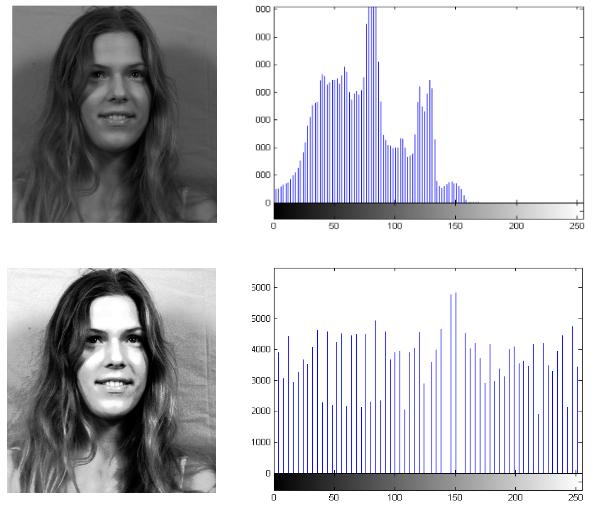
\includegraphics[width=300.0pt]{graphics/img/he/1.png}
%   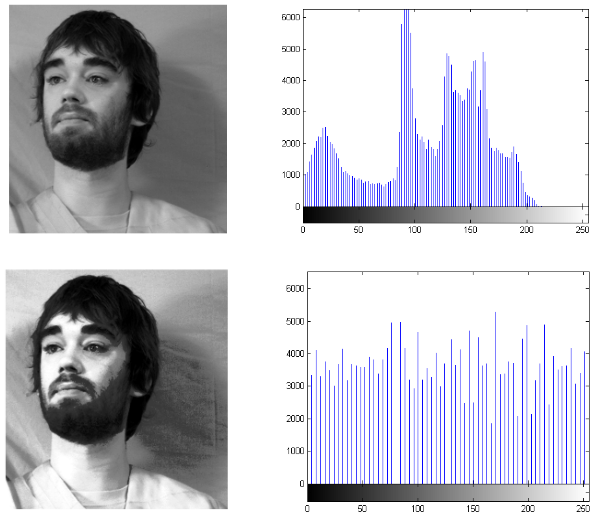
\includegraphics[width=300.0pt]{graphics/img/he/2.png}
%   \caption{Результаты нормировки интенсивности пикселей изображения}
%   \label{fig:histogram_equalization}
%   \stepcounter{myfigure}
% \end{figure}

Несмотря на то, что нормировка гистограммы изображения в большинстве случаев позволяет добиться требуемых результатов, в ряде случаев невозможно получить равномерно распределенную гистограмму. Наличие теней на изображении, зашумленость и другие причины приводят к тому, что в результате нормировки значения гистограммы не распределяются по всему диапазону возможных интенсивностей.


Метод связанных компонент применяется для нахождения связанных областей на изображении. Данный метод может быть использован, например, для нахождения областей, окрашенных в телесный цвет. После процедуры разбиения изображения на отдельные области производится поиск области, которая отображает лицо человека, среди всех выделенных телесных областей.

Алгоритм нахождения связанных компонент может быть представлен следующими шагами:

\begin{enumerate}
	\item Задание правил, по которым пара пикселей относится к одной и той же области.
	\item Осуществление просмотра и анализа пикселей изображения.
	\item Для каждого пикселя $p$ проверяется его схожесть с окружающими его соседними пикселями (сверху и слева). Если ни один из соседних пиксель не удовлетворяет определенным правилам, то рассматриваемый пиксель помечается специальной меткой, которая соответствует новой области. Если только один соседний пиксель удовлетворяет всем критериям, то рассматриваемому пикселю присваивается метка соседа. Если оба соседа удовлетворяют всем критериям и имеют одинаковые метки, то данная метка также присваивается рассматриваемому пикселю. В противном случае, если оба соседа удовлетворяют всем правилам, но имеют отличные метки, то анализируемому пикселю присваивается любая метка, но обе метки добавляются в один класс эквивалентности. 
	\item После просмотра всех пикселей, осуществляется повторный просмотр, с целью распределить пиксели по классам эквивалентности. Если метка пикселя принадлежит к определенному классу эквивалентности, то создается новая общая метка, которая присвается всем пикселям данного класса.
\end{enumerate}

Существует множество факторов, влияющих на производительность и качество алгоримта нахождения связанных компонент. Wu et al. (2005) в своей работе рассмотрели возможные способы оптимизации данного алгоритма. В итоге авторами были предложены структуры данных, использование которых позволяет добиться производительности достаточной для работы в реальном режиме времени.


\subsection{Автоматическая обработка изображений человеческого лица}

В данной главе производится описание существующих исследований и технических аспектов, которые используются при автоматической обработке изображений человеческих лиц.


Связь подсистемы автоматической обработки человеческих лиц с другими подсистемами представлена на рисунке \ref{fig:sstructure}. Обобщенная процедура автоматического анализа человеческого лиц апредставлена на рисунке \ref{fig:face-analyse-structure}

\begin{figure}
  \centering
  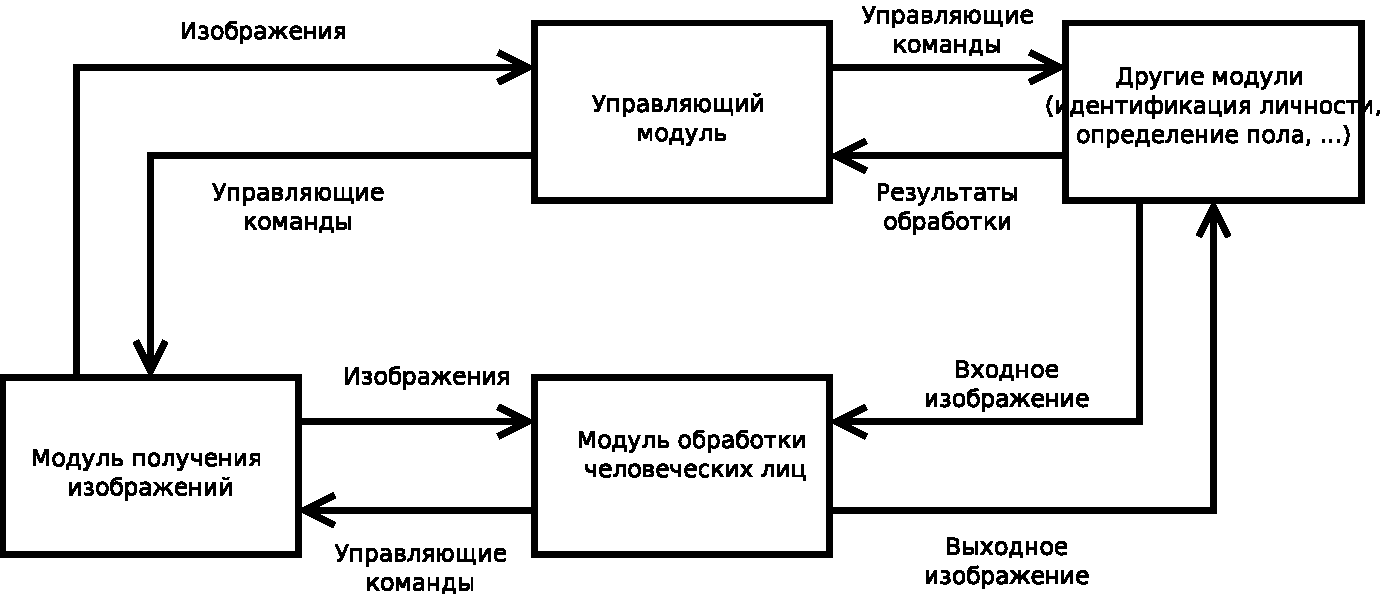
\includegraphics[width=\textwidth]{inc/dia/face-analyse-relation}
  \caption{Обобщенная структура модулей в системе распознавания человеческих лиц}
  \label{fig:sstructure}
\end{figure}

\begin{figure}
  \centering
  
\includegraphics[width=\textwidth]{inc/dia/face-analyse}
  \caption{Обобщенная структура модулей в системе распознавания человеческих лиц}
  \label{fig:face-analyse-structure}
\end{figure}

Из рисунка \ref{fig:sstructure} видно, что управляющий модуль контролирует работу всей системы с помощью выдачи команд другим модулям.
Модуль получения изображений предоставляет изображения, например,  захватывая их с видеокамер, и управляющая программа может выводить результат пользователю.
Компонент автоматической обработки изображений для выделения человеческих лиц осуществляет обработку входных изображений и предоставляет результаты управляющему модулю.
Результатами могут являться:

\begin{enumerate}
  \item количество и позиции обнаруженных лиц;
  \item описание выражений обнаруженных лиц;
  \item гендерная классификация обнаруженных лиц;
  \item идентификация обнаруженных лиц.
\end{enumerate}


Модулю, предоставляющему изображения, могут посылать команды как управляющий так и анализирующий модули. Также в системах компьютерного зрения могут присутствовать и другие модули такие как:

\begin{enumerate}
  \item модуль распознавания речи;
  \item отслеживания перемещений объектов.
\end{enumerate}

Данные модули взаимодействуют с анализирующим модулем и производят дополнительную обработку для наделения обнаруженных объектов дополнительными свойствами, которые впоследствии отсылаются управляющей программе. Дополнительная информация об объекте может быть использована управляющей программой для более точного решения поставленных задач. Например, процедура идентификации человека может быть основана на информации о лице человека и его речи.





На рисунке \ref{fig:face-analyse-structure} показаны общие этапы процедуры автоматической обработки человеческих лиц на изображениях. Первым этапом процедуры является его локализация человеческого лица. В зависимости от целей приложения объект лица может отслеживаться на некоторой последовательности кадров, а может опеределяться обработкой одиночного изображения. Целью автоматической обработки человеческого лица является определение присутствия на входном изображении какого-либо количества человеческих лиц и их локализация. Отслеживание человеческого лица (tracking) означает определение траектории движения целевого объекта на последовательности кадров видеопотока. Выделение особенностей человеческого лица означает определение по изображению лица расположение глаз, носа, рта и других частей лица, в зависимости от решаемой задачи. Результаты первого этапа могут использоваться в первоначальном виде, однако в большинстве случаев применяют процедуру нормализации. Целью является снижение влияния на изображение различного освещения. Нормализованное изображение может подвергаться процедуре классификации. Однако осуществляется подготовительный этап --- составления входного вектора для классификатора. В простейшем случае таким ветором может являться последовательный набор пикселей исследуемого изображения.

Этап классификации может решать несколько задач. Например, определение пола, возраста, рассовой принадлежности, эмоций. Задачи могут решаться полностью самостоятельно, но иногда более выгодно последовательное решение задач. Так, например, если задачи определения пола, возраста и рассовой принадлежности предшествуют процедуре идентификации личности, то скорость распознавания может быть увеличена в несколько раз так как сужаются границы поиска.


Основным требованием к алгоритмам автоматической обработки человеческих лиц является скорость и точность работы. Алгоритмы не должны являться сложными с вычислительной точки зрения.



\subsection{Обнаружение и слежение за человеческими лицами}

Автоматическое обнаружение человеческих лиц означает поиск человеческих лиц на изображении, трэкинг лиц --- отслеживание положния каждого лица на последовательности кадров.


Процедура автоматической детекции человеческих лиц на изображениях является сложной задачей в связи с множеством возникающих проблем. Так каждый человек имеет уникальное лицо, это означает, что на изображениях лица также будут выглядеть неодинаково. Более того лицо отдельно взятого человека может выглядеть по-разному в зависимости от освещенности, времени года и других факторов. Наличие солнцезащитных очков, усов, бороды, макияжа является также фактором, усложнгяющим процедуру детекции. Также может меняться  положение лица в пространстве сцены и его ориентация. Наиболее влиятельным фактором является изменение параметров самого изображения: проблема различного освещения, разрешения изображений, цветовой модели, зашумленность изображений.

Обнаружение лиц на изображении является начальным этапом в процедуре автоматической обработки и анализа человеческих лиц, поэтому данная тема получила широкую популярность среди ученых в области компьютерного зрения. С этой точки зрения оценка методов обнаружения человеческих лиц является очень важной. В настоящее время существуют свободно распространяемые базы данных для проведения подобных оценок. 

Множество исследований посвящены составлению оценочных баз данных, включающих изображения с множеством лиц в различных условиях (Yang et al., 2002): 

\begin{enumerate}
	\item комбинированный набор лиц, содержащий их фронтальные изображения, предложенный Sung, Poggio, Rowley, Baluja (Sung and Poggio, 1998; Rowley et al., 1998a; Rowley et al., 1998b);
	\item набор профилей человеческих лиц подготовленный учеными университета Карнеги — Меллон (Schneiderman and Kanade, 2000);
	\item ученые Sharma и Reilly из Дублинского университета  составили базу цветных изображений человеческих лиц (Sharma, Reilly, 2003).
\end{enumerate}

В качестве мер для оценки детекторов человеческих лиц принято использовать:
\begin{enumerate}
	\item точность определения;
	\item скорость определения;
	\item время, требуемое для обучения классификаторов;
	\item количество изображений необходимых для обучения классификаторов;
	\item требования к памяти в процессе обучения и использования.
\end{enumerate}

Точность детектирования определяется частотой верных и ложных обнаружений. Частота верных обнаружений определяется как отношение количества верно обнаруженных лиц к общему количеству лиц на изобрежнии. Аналогично определяется частота ложных срабатываний --- отношение количества ложных срабатыванийдетектора к общему количеству лиц на изображении. Также общеприняты следующие количественные меры для оценки качества работы алгоритмов детектирования объектов на изображениях:

\begin{enumerate}
	\item FP (false positives) --- количество объектов изображения, ложно принятых за человеческие лица;
	\item FN (false negatives) --- количество человеческих лиц на изображении, которые не были обнаружены. 
\end{enumerate}

Для наглядного сравнения различных алгоритмов, решающих задачу бинарной классификации, к которой можно отнести задачу детектирования человеческих лиц, строят так называему кривую ошибок (ROC-кривую (Receiver Operating Characteristics)). ROC-кривая показывает зависимость между частотой верных положительных классификаций и ложных положительных классификаций. На рисунке \ref{fig:ROCsample} приведен пример сравнения результатов работы алгоритмов, которые были исследованы в работе (cite Huang, 2007). ROC-кривая монотонно не убывает. Чем выше лежит кривая, тем лучше качество классификации.

Несомненно высокая частота верных положительных классификации при отсутсвии ложных детекций является предпочтительной. Однако в некоторых случаях в зависимотси от предметной области и задачи, в рамках которой осуществляется определение человеческих лиц, этот показатель может меняться. Например, в своей работе (cite Yang) описывает решение задачи идентификации человека по изображению лица. После локализации изображения лиц сравниваются с изображениями, хранящемися в базе данных. В данном случае большое количество ложных положительных классификаций не является критичиным, так как данные изображения будут отсеяны при попытке найти совпадения в базе данных.

Другим важным показателем является скорость работы детектора человеческих лиц. Одним из факторов, влияющих на скорость работы, является размер обрабатываемых изображений. Очевидно, что чем больше изображение, тем больше времени требуется для его обработки и локализации человеческих лиц. Другим не менее важным фактором являются характеристики аппаратного обеспечения. Наиболее частым требованием к приложениям является обеспечение возможности работать в реальном режиме времени. Из подходящих алгоритмов в таком случае можно выделить алгоритм Виолы-Джонса, использующий каскадный классификатор Хаара (cite Viola-Jones). С развитием аппаратных мощностей могут применяться также алгоритмы, требующие значительно больших вычислительных ресурсов и мощностей.

Размер обучающей выборки важен с точки зрения требований к затратам памяти для обучающихся систем. Время обучения также является критичным для приложений, работающих в реальном режиме времени и требующими обновление обученной базы (Yang 2002).

\subsection{Оценка полученных результатов}
Одной из проблем, которую приходится решать при обработке результатов детектора человеческих лиц, --- точность, с которой должно быть определена позиция лица на изображении. На рисунке \ref{fig:difffaces}, которую приводит в своей работе Yang (cite Yang, 2002), представлены обрабатываемое изображение и результаты обнаружения. Из всего набора выходных результатов необходимо выбрать один или несколько, наиболее подходящие для решения поставленных заадач. 

В своих исследованиях Yang провел обширный обзор существующих алгоритмов автоматического определения человеческих лиц (cite Hjelmas and Low, 2001; Yang, 2002). Исследуемые алгоритмы могут быть подвержены классификации. Yanfg выделяет следующие группы методов: основанные на правилах (knowledge-based), основанные на выделении инвариантных особенностей объектов(feature invariant), основанные на сопоставлении шаблонов (template matching) и базирующиеся на применении алгоритмов машинного обучения (нейронные сети, SVM, AdaBoost).

В методах первого типа используются наборы правил, которые задаются с помощью взаимодействия с пользователями. Эти правила формируются согласно знаниям о геометрии челоческого лица. Примеры систем основанных на использовании данного подхода приведены в работах (cite Sobottka and Pitas,1196; Makinen and Raisamo,2002; Castrillon-Santana, 2003). Например, следующие выражения могут быть использованы в качестве правил: <<глаза располагаются в верхней части середины головы>>, <<отношение расстояния между глаз к ширине головы должно находиться в определенном диапазоне>>. Правила могут быть также основаны на характеристиках самого изображения, например, распределению интенсивности: <<левому и правому глазу соответствует значительное снижение интенсивности (минимум)>>(cite Sobottka and Pitas, 1996). 



\section{Обзор существующих алгоритмов}

Существующие алгоритмы обнаружения лиц можно разбить на две категории. К
первой категории относятся методы, отталкивающиеся от опыта человека в
распознавании лиц и делающие попытку формализовать и алгоритмизовать этот опыт,
построив на его основе автоматическую систему распознавания. Вторая категория
опирается на инструментарий распознавания образов, рассматривая задачу
обнаружения лица, как частный случай задачи распознавания. 

В дальнейшем согласно \cite{Veznevec_Degtyareva} алгоритмы первой категории
будем относить к эмпирическому распознаванию, второй --- к моделированию
изображения лица. Авторы \cite{Veznevec_Degtyareva} в своей работе приводят
наиболее полную классификацию данных алгоритмов.

\subsection{Эмпирическое распознавание}

Авторы алгоритмов данного типа стремились использовать принципы, которыми
руководствуется человеческий мозг при решении задачи распознавания образов.
Выделяют два направления методов данной категории: основанные на знаниях и
основанные на особенностях.

Распознавание, основанное на знаниях, заключается в построении набора правил, с
помощью которого будет найден фрагмент изображения, являющийся
человеческим лицом. Например, одними из правил могут быть правила симметрии
лица (глаза, брови), пигментации губ и так далее, расположения определенных
черт лица. Алгоритм заключается в проверке всех фрагментов изображения на
выполенение всех правил.

Улучшенной модификацией данного класса алгоритмов являются
шаблонно-ориентиованные алгоритмы. Пользователем заранее создаются наборы, так
называемых шаблонов, с которыми производится сранение фрагментов изображения.
Фактически одного сравнения достаточно для определения является ли данный
фрагмент человеческим лицом или нет.

Другой класс алгоритмов распознавания основывается на выделении особенностей,
то есть инвариантных свойств изображений человеческого лица, что позволяет
отделить его от фона и других объектов сцены.

В качестве инвариантных свойств выделяют:
\begin{enumerate}
 \item границы (ребра) объектов;
  \item цвет (кожа);
  \item форма черт лица (форма губ, овала лица и так далее);
  \item комбинированные свойства.
\end{enumerate}

Следующим шагом алгоритмов данного класса является определение областей со
связными особенностями и их проверка на соответствие изображению человеческого
лица. 

Принцип заложенный в данном подходе получил популярность у многих ученых:
\begin{enumerate}
 \item K. Sobottka в своей диссертации \cite{K_Sobottka} предложил выделять
инвариантные свойства на основе их яркости в предположении, что такие черты
лица как губы, глаза, брови, имеют низкую яркость в отличие от окружающих
частей лица;
  \item F. Smeraldi реализовал алгоритм \cite{F_Smeraldi}, использующий
положение глаз для локализации человеческого лица. 
\end{enumerate}


\subsection{Моделирование изображения лица}
Основной задачей алгоритмов данной категории является построение математической
модели человеческого лица, применяя методы математической статистики и
машинного обучения.

В общем случае фрагменту изображения ставится в соответствие некоторым образом
вычисленый вектор признаков, который используется для классификации изображения
на два класса --- лицо, либо не лицо.

В алгоритмах данного типа используются:
\begin{enumerate}
  \item моделирование класса изображений лиц с помощью Метода Главных Компонент;
  \item моделирование класса изображений лиц с помощью Факторного анализа;
  \item Линейный Дискриминантный Анализ (Linear Discriminant Analysis, LDA);
  \item нейронные Сети (Neural Networks, NN);
  \item скрытые Марковские Модели (Hidden Markov Models, HMM);
  \item Sparse Network of Windows (SNoW);
  \item Active Appearance Models (AAM).
\end{enumerate}

Для классификации фрагментов в основном используют метод опорных векторов.

Входными данными для перечисленных алгоритмов является поток цифровых
изображений.

Под цифровым изображением при реализации данных алгоритмов понимается случайный
двумерный дискретный сигнал, наблюдаемый системой. Последовательность
наблюдений, то есть вектор наблюдений может извлекаться из изображения
различными способами. В силу этого описательные способности полученных моделей
могут различаться. Наиболее популярным является вариант сканирования изображения
прямоугольным окном. Для уменьшения вероятности потери данных на границах
блоков, сканирование изображений осуществляется таким образом, что соседние
блоки пикселей перекрываются друг другом. Значение перекрытия задается в
качестве параметра алгоритма.

Для снижения вычислительной сложности и уменьшения пространства признаков,
каждый извлеченный блок пикселей подвергается некоторому преобразованию, в
результате которого получается некоторый набор числовых данных, который и
является вектором наблюдений.

В каждом алгоритме используется конкретный математический аппарат, позволяющий
справиться с поставленной задачей локализации человеческого лица.

//TODO: более полное описание существующих алгоритмов. VIOLA-JHONES.

\subsection{Сравнительный анализ}

К недостаткам эмпирического подхода можно отнести высокую чувствительность
алгоритма к изменчивости объекта распознавания, зависимость от условий съемки и
освещения.

Несомненным достоинством является то, что применение эмпирических правил
позволяет снизить сложность проверок при обработке изображения для локализации
лиц.

В целом основной трудностью при реализации алгоритмов эмпирического типа
является сложность построения эмпирических правил: поскольку чересчур жесткие
рамки правил приведут к тому, что в ряде случаев лица не будут обнаружены, и
напротив, слишком общие правила приведут к большому количеству случаев ложного
обнаружения. 

Основанные на классификаторах алгоритмы второй категории чувствительны к
изменениям ориентации и масштаба лица, так как большинство из классификаторов
не являются инвариантными к повороту лица и изменению его размера. Это приводит
к необходимости в предварительной обработке входного изображения:
масштабирование, поворот, перспективные преобразования; либо составлению более
полного тренировочного набора. В целом алгоритмы второй категории обладают
более высокой вычислительной сложностью, что затрудняет использование некоторых
из них в системах реального времени.


К общим трудностям многих алгоритмов обеих категорий можно отнести
восприимчивость к повороту лиц вне плоскости изображения. Правила алгоритмов
эмпирического типа в данном случае становятся совершенно непригодными.

Несмотря на наличие общих недостатков в алгоритмах обеих категории, существуют
методы позволяющие снизить влияние негативных факторов на результат
обнаружения. Например, проблему разницу в освещении, масштабирования решают
предварительной обработкой входного изображения.

В итоге можно сделать вывод, алгоритмы, использующие эмпирический подход,
просты в реализации и их целесообразно использовать для задач реального времени
с некритичными требованиями к точности обнаружения. Алгоритмы, основанные на
моделировании изображения лица, сложны в реализации, не всегда могут быть
применимы в задачах реального времени, однако позволят достичь более
высокой точностью обнаружения.

\section{Определение пола и возраста человека по изображению лица}
В своих работах многие ученые освещали способы решения проблемы, связанной с
обработкой изображений для определения пола и возраста человека. Авторы
предлагют различные методы такие как: метод опорных векторов, методы, основанные
на геометричеких особенностях, графовых моделях и методы на основе нейронных
сетей. В данной главе производится обзор различных подходов к решаемой проблеме:
подходе основанном на выделении геометрических особенностей и подходе на основе
шаблонов.


\subsection{Геометрический анализ}
Представление лиц  с точки зрения геометрических особенностей является самым
распространенным методом решения задач обработки лиц. Обычно выделяются
геометрические особенности инвариантные к  масштабированию, перспективным
искажениям и поворотам такие как расстояния, углы и отношения между частями
лица. Эти особенности представляют человеческое лицо и обеспечивают входные
данные для обучения классификатора, который осуществляет окончательную
классификацию.

Bruneli и Poggio \cite{Bruneli_Poggio} использовали данный подход в своих
работах для определения пола человека. Их алгоритм предполагает извлечение из
изображения лица человека шестнадцати геометрических особенностей. Впоследствии
эти данные используются для обучения двух различных классификаторов, отдельно
для мужчин и женщин. Описанный в \cite{Bruneli_Poggio} алгоритм позволяет
добиться 90\% точности распознавания для изображений из обучающего набора и 79\%
для новых изображений.

Первым этапом в любом алгоритме, основанном на геометрических параметрах объкта
распознавания, является извлечение характеристических особенностей из входного
изображения. В своей работе \cite{Yang_Huang} Yang и Huang описывают метод
основанный на иерархическом обучении для определения лиц людей на изображениях,
представляющих сложные динамические сцены с множеством других объектов.
Shackleton и Welsh \cite{Shackleton_Welsh} разработали алгоритм, позволяющий с
высокой точностью выделять глаза на фронтальном изображении лица человека. Wu и
Yokoyama \cite{Wu_Yokoyama} предоставляют основанный на информации о цвете
алгоритм, с помощью которого можно выделять различные геометрические черты лица
человека. В работе Eveno, Caplier и Coulon \cite{Eveno_Caplier_Coulon}
описывается алгоритм, выделения формы губ. Данный алгоритм основан на цветовой
информации и требует обучения с помощью входного множества цветных изображений
губ людей.


\subsection{Классификация с использованием специфических особенностей объекта}

В настоящее время создано множество приложений, базирующихся на выделении из
изображений лица таких специфических особенностей, как усы, борода и другие.
Применение подобной методики позволяет быстро отсеять точно неподходящие
варианты. Например, солжно представить женщину с бородой.

Lapedriza, Masip и Vitria \cite{Lapedriza_Masip_Vitria} предложили алгоритм,
основанный на низходящей обработке изображения для выделения специфических
особенностей. Процесс обучения в данном алгоритме отличается от рассмотренных
ранее тем, что обучаются лишь те участки изображения, в которых могут
присутствовать интересующие нас объекты. С использованием данного алгоритма
удалось добиться показателя точности 94\% для обучающей выборки из 90
изображений лиц (40 мужских, 40 женских).


\subsection{Нейронные сети}
Многие ученые для решения рассматриваемой задачи используют нейронные сети.
Colomb \cite{Colomb} предложил использовать нейронную сеть с обратной связью
размером $900\times40\times900$. В описанном алгоритме обрабатываемые
изображения преобразуются к размеру $30\times30$, также производится поворот
изображения так, чтобы на всех изображениях обучающей выборки позиции глаз и губ
были идентичны. На выходе сеть выдает $1$ --- если детектирован мужчина и $0$
--- если определена женщина. Средняя ошибка алгоритма \cite{Colomb} составляет
$8,1\%$.  

\subsection{Метод опорных векторов}
Метод опорных векторов (SVM, Support Vector Machine) является алгоритмом вида
<<обучения с учителем>> и используется для задач классификации и регрессионного
анализа. Основная идея метода опорных векторов --- перевод исходных векторов в
пространство более высокой размерности и поиск разделяющей гиперплоскости с
максимальным зазором в этом пространстве. 

Babac в своей работе \cite{Babac} провел исследование и установил, что
классификатор SVM является наиболее точным для изображений с низким
разрешением.


\subsection{Выбор алгоритма}
Авторы \cite{Veznevec_Degtyareva} предлагают осуществлять выбор алгоритма
обнаружения и локализации лиц на изображениях в соответствии со схемой
представленной в таблице \ref{tab:chose_algo}.

\begin{table}[ht]
  \caption{Выбор алгоритма обнаружения и локализации лиц на изображениях}
  \begin{tabular}{|p{0.25\textwidth}|p{0.70\textwidth}|}
  \hline
  Параметр & Значение \\ 
  \hline
  Предполагаемое разнообразие лиц & Ограниченный набор людей, ограничения на
возможный тип лица, отсутствие ограничений. \\ 
  \hline
  Ориентация лиц на изображении & Наклон под известным
углом, в определенных границах вблизи известного угла наклона, любая
ориентация. \\
  \hline
  Цветовая палитра & Цветное или черно-белое избражение. \\
  \hline
  Количество лиц & Фиксировано, неизветно. \\
  \hline
  Фон & Фиксированный, контрастный однотонный, слабоконтрастный зашумленный,
неизвестный. \\
  \hline
  Условия освещения & Фиксированные известные, приблизительно известные, любые.
  \\
  \hline
  \end{tabular}
  \label{tab:chose_algo}
\end{table}

Помимо этого авторы акцентируют внимание на таких параметрах как качество
обрабатываемых изображений, а также точности желаемого результата. В некоторых
задачах важно не пропустить ни одного лица, но допускаются случаи ложного
обнаружения. В других случаях возможны более строгие требования именно к
качеству обнаружения, для этого необходимо минимизировать количество случаев
ложного обнаружения.

Стоит отметить, что предложенная схема также подходит для задачи более высокого
уровня, то есть определения пола и возраста человека по изображению лица.

Из рассмотренных примеров видно, что некоторые характеристики объектов сцены
с одной стороны позволяют более эффективно устанавливать пол человека, а с
другой затруняют локализацию лица на изображении, например, к таким
характеристикам можно отнести усы и бороду.




\section{Выводы}
Многие ученые посвятили свои труды решению проблемы обработки изображений с
целью определения пола и возраста человека. Было установлено, что разработанные
на данный момент решения хотя и предоставляют относительно высокие показатели
точности, должны быть соотнесены с конкретной сферой применения для решения
конкретных задач.


%%% Local Variables: 
%%% mode: latex
%%% TeX-master: "rpz"
%%% End: 

%\chapter{Конструкторская часть}
\label{cha:design}


\section{Вступление}
Одной из областей компьютерного зрения ялвяется --- анализ человеческого лица по цифровому изображению.
Большинство существующих алгоритмов настолько ресурсоемки, что время их выполенения достаточно медленное для того, чтобы решать задачи в реальном режиме времени.
Однако с улучшением аппаратной базы, увеличением частоты процессора, данная проблема становится менне значимой (Piccardi and Jan, 2003).
На передний план выходит проблема, связанная с тем, что на данный момент не существует надежного алгоритма, который одинаково справлялся бы с большинством задач.

Например, комерческие разработки для идентификации личности, основанные на распознавании частей лица, имеют множество ограничений (Pentland, 2000). 

Такие области науки как распознавание образов по шаблонам и машинное обучение тесно связаны с областью компьютерного зрения. Алгоритмы распознавания и машинного обучения часто применяются в качестве составляющих в алгоримах компьютерного зрения. К примеру, существует множество алгоримов для выделения из видеопотока человеческих лиц и их анализа использхующих нейронные сети (Abdi et al., 1995; Golomb et al., 1990; Gray et al., 1995; Huang and Shimizu, 2006; Rowley et al., 1998; Tamura et al., 1996), Adaboost (Huang et al., 2004; Shakhnarovich et al., 2002; Sun et al., 2006; Viola and Jones, 2001; Wu et al., 2003), скрытые марковские модели (СММ) (Aleksic and Katsaggelos, 2006; Kohir and Desai, 1998; Yin et al., 2004), метод опорных векторов (SVM — support vector machines) (BenAbdelkader and Griffin, 2005; Castrillon-Satana et al., 2005; Moghaddam and Yang, 2000; Saatci and Towm, 2006; Sun et al., 2002; Yang et al., 2006).

В рамках компьютерного зрения анализ человеческого лица применяется для решения следующих задач:


\begin{itemize}
	\item обнаружение лица в видеопотоке и его отслеживание;
	\item идентификация личности;
	\item определение пола;
	\item определение возраста;
	\item определение эмоций;
	\item распознавание жестов;
	\item определение этнической принадлежности.
\end{itemize}

Несмотря на огромный прогресс достигнутый учеными за последние годы, решение для многих проблем так и не было предложено. Например, до сих пор не разработана система, которая бы позволила осуществлять обнаружение лиц и надежно идентифицировать по ним личность человека во всех возможных положениях лица. Фронтальное изображение лица в значительной степени отличется от изображения профиля, также возможны различные перспективные искажения, в том числе играют роль условия освещенности. Стоит отметить, что иногда возможны случаи, когда определить личность по изображению лица крайне трудно или вообще невозможно даже самим человеком.



В данной главе производится описание процесса распознавания образов человеческим зрением, также производится обзор подходов к цифровой обработке изображений, примение алгоритмов машинного обучения и алгоритмов распознавания образов.

\section{Человеческое зрение}
Для понимания проблем компьютерного зрения и автоматической обработки человеческих лиц полезно узнать процесс распознавания образов человеческим зрением.

В своем исследовании Tsao (2006) показал, что специальные клетки мозга чувствительны к воспринятию отдельных черт лица. В своих экспериментах авторы использовали лица, состоящие из картонных элементов. Изменяя положение девятнадцати составляющих, включая, положение глаз, носа, губ, размеры головы, ученые исследовали активность клеток головного мозга подопытных макак. В результате ученые выяснили, что одна клетка мозга восприимчива к изменению положения восьми составляющих. Также ученые выделили некоторые составляющие, изменение которых приводило к наибольшей активности отдельных секторов мозга.

\begin{figure}
\label{}
\end{figure}

Очевидно, что процесс распознавания образов с помощью человеческого зрения достаточно сложен и до конца не изучен. Сложность компьютерного зрения обуславливается анализом изображений, получаемых устройством захвата: разбиение входных изображений на отдельные части, объединение частей для получения смысловых элементов, и определение значения полученных элементов. Понятие процессов происходящих при человеческом зрении многим ученым позволило применить используемые в них правила и подходы для разработки алгоритмов компьютерного зрения.

\section{Компьютерное зрение}
Область компьютерного зрения весьма обширна. Применения находят как и промышленные приложения, так и приложения для домашнего использования. Однако, многие основные процессы и технологии являются одинаковыми при разработке приложений для различных сфер. В этой главе производится обзор этих подходов. Цифровая обработка изображений --- базис для дальнейшей обработки более высокого уровня, такой как распознавание образов. Также рассматриваются методы машинного обучения и распознавания образов, так как они получили широко применение в сфере компьютерного зрения.

\subsection{Цифровая обработка изображений}
Цифровая обработка изображений является базисной для всех систем компьютерного зрения. Существует несколько способов обработки изображений.

Цифровые камеры оснащаются либо КМОП (комплементарная логика на транзисторах металл-оксид-полупроводник), либо CCD-матрицами, которые преобразуют входной световой поток и преобразует его в разницу напряжений. Захват светового потока осуществляется с помощью светочувствительных датчиков. Количество датчиков зависит от типа камеры. Стандартные веб-камеры имеют размер матрицы 640*480. В настоящее время существуют камеры, оснащенные CCD-матрицами размером до 6 МегаПикселей.  

После преобразования светового потока в разницу напряжений происходит так называемое квантование. Это означает, что напряжение в определенном диапазоне отождествляется со строго определенным значением. Итогом процедуры квантования является изображение, представленное в цифровом виде, которое может в дальнейшем быть сохранено для последующей обработки.

Низкоуровневая обработка изображений может включать в себя фильтрацию в пространственной и частотной области. Основной задачей низкоуровневой обработки является улучшение качества изображения (Gonzalez and Woods, 2002, pp. 25-28). Также могут применяться процедуры морфологической обработки изображений и из сегментации на составляющие части.

Одной из задач фильтрации входных изображений является получение фильтрованного изображения, в котором интенсивности всех пикселей растянуты на более широком диапазоне. Применение подобной фильтрации позволяет снизить влияние таких факторов как ошибки в калибровке камеры, а также повысить контрастность изображения (Rowley et al., 1998). В рамках задачи анализа человеческого лица очень важно снизить влияние внешних условий на изменение изображения лица.

Преобразование гистограммы исходного изображения для усреднения интенсивностей является просто реализуемым. Для получения гистограммы применяют формулу:


%%% Local Variables:
%%% mode: latex
%%% TeX-master: "rpz"
%%% End:

%\chapter{Технологический раздел}
\label{cha:impl}

В данном разделе описано изготовление и требование всячины. Благодаря пакет \Code{underscore} эскейпить подчёркивание  не нужно (\Code{some_function}).

Для вставки кода есть пакет \Code{listings}. К сожалению, пакет \Code{listings} всё ещё
работает криво при появлении в листинге русских букв и кодировке исходников utf-8.
В данном примере он (увы) на лету конвертируется в koi-8 в ходе сборки pdf.

Есть альтернатива \Code{listingsutf8}, однако она работает лишь с
\texttt{\textbackslash lstinputlisting}, но не с окружением \Code{lstlisting}

Вот так можно вставлять псевдокод (питоноподобный язык определен в шаблоне):

\begin{lstlisting}[style=pseudocode,caption={Алгоритм оценки дипломных работ}]
def EvaluateDiplomas():
    for each student in Masters:
        student.Mark := 5
    for each student in Engineers:
        if Good(student):
            student.Mark := 5
        else:
            student.Mark := 4
\end{lstlisting}

Еще в шаблоне определен псевдоязык для BNF:

\begin{lstlisting}[style=grammar,basicstyle=\small,caption={Грамматика}]
  ifstmt -> "if" "(" expression ")" stmt |
            "if" "(" expression ")" stmt1 "else" stmt2
  number -> digit digit*
\end{lstlisting}

В листинге~\ref{lst:sample01} работают русские буквы. Сильная магия. Однако, работает
только во включаемых файлах, прямо в \TeX{} нельзя.

% Обратите внимание, что включается не ../src/..., а inc/src/...
% В Makefile есть соответствующее правило для inc/src/*,
% которое копирует исходные файлы из ../src и конвертирует из UTF-8 в KOI8-R.
% Кстати, поэтому использовать можно только русские буквы и ASCII,
% весь остальной UTF-8 вроде CJK и египетских иероглифов -- нельзя.

\lstinputlisting[language=C,caption=Пример (\Code{test.c}),label=lst:sample01]{inc/src/test.c}

% Для вставки реального кода лучше использовать \texttt{\textbackslash lstinputlisting} (который понимает
% UTF8) и стили \Code{realcode} либо \Code{simplecode} (в зависимости от размера куска).




Можно также использовать окружение \Code{verbatim}, если \Code{listings} чем-то не
устраивает. Только следует помнить, что табы в нём <<съедаются>>. Существует так же команда \Code{verbatiminput} для вставки файла.

\begin{verbatim}
a_b = a + b; // русский комментарий
if (a_b > 0)
    a_b = 0;
\end{verbatim}

%%% Local Variables:
%%% mode: latex
%%% TeX-master: "rpz"
%%% End:

%\chapter{Экспериментальный раздел}
\label{cha:research}

В данном разделе проводятся вычислительные эксперименты.
А на рис.~\ref{fig:spire01} показана схема мыслительного процесса автора...

\begin{figure}
  \centering
  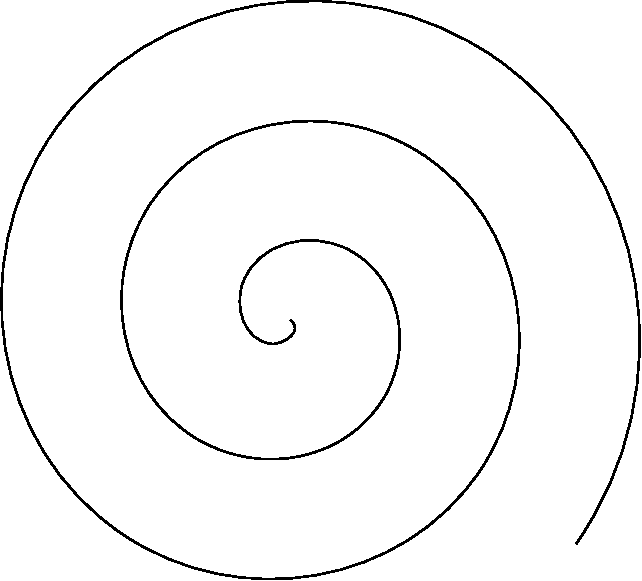
\includegraphics[width=\textwidth]{inc/svg/pic01}
  \caption{Как страшно жить}
  \label{fig:spire01}
\end{figure}


%%% Local Variables:
%%% mode: latex
%%% TeX-master: "rpz"
%%% End:


\backmatter %% Здесь заканчивается нумерованная часть документа и начинаются ссылки и
            %% заключение

%\Conclusion % заключение к отчёту

В ходе работы был осуществлен обзор существующих алгоритмов локализации
человеческих лиц на изображении и определения пола и возраста человека:
основанных на геометрических особенностях объектов изображений и базирующихся на
текстурных шаблонах изображения, цветовых характеристиках. Также были
рассмотрены различные методологии и подходы применяемые для достижения цели
работы: использование нейронных сетей и метода опорных векторов. 

Существующие решения позволяют добиться относительно высоких показатели
точности, но в значительной степени зависят от области применения. Поэтому для
дальнейшей работы были выделены следующие этапы:

\begin{enumerate}
\item определение области применения;
\item осуществление подробного анализа существующих алгоритмов;
\item анализ ключевых точек и установление инвариантных особенностей
человеческого лица;
\item сравнение существующих алгоритмов, выделение их достоинств и недостатков; 
\item проведение экспериментов с целью определения подходящих алгоритмов;
\item измерение показателей точности и быстродействия алгоритмов;
\item синтез алгоритма обработки изображений для определения пола и возраста
человека.
\end{enumerate}


%%% Local Variables: 
%%% mode: latex
%%% TeX-master: "rpz"
%%% End: 


% % Список литературы при помощи BibTeX
% Юзать так:
%
% pdflatex rpz
% bibtex rpz
% pdflatex rpz

\bibliographystyle{gost780u}
\bibliography{rpz}

%%% Local Variables: 
%%% mode: latex
%%% TeX-master: "rpz"
%%% End: 


\appendix   % Тут идут приложения

%\chapter{Картинки}
\label{cha:appendix1}

\begin{figure}
\centering
\caption{Картинка в приложении. Страшная и ужасная.}
\end{figure}

%%% Local Variables: 
%%% mode: latex
%%% TeX-master: "rpz"
%%% End: 

%\chapter{Еще картинки}
\label{cha:appendix2}

\begin{figure}
\centering
\caption{Еще одна картинка, ничем не лучше предыдущей. Но надо же как-то заполнить место.}
\end{figure}

%%% Local Variables: 
%%% mode: latex
%%% TeX-master: "rpz"
%%% End: 


\end{document}

%%% Local Variables:
%%% mode: latex
%%% TeX-master: t
%%% End:
